% !TeX encoding = UTF-8
% !TeX spellcheck = de_DE

\documentclass[9pt]{beamer}
\usetheme{metropolis}
\usepackage{iftex}

\ifPDFTeX
\usepackage[T1]{fontenc}
\usepackage[utf8]{inputenc}
\usepackage{lmodern}
\usepackage{amsmath,amsfonts,amssymb}
\fi

\ifXeTeX
\fi

\ifLuaTeX

\fi

\usepackage[ngerman]{babel}

%\beamerdefaultoverlayspecification{<+->}


%\setsansfont[BoldFont={Fira Sans SemiBold}]{Fira Sans Book}
%\setsansfont{libertine}
%\setmonofont{Helvetica Mono}

\usepackage{appendixnumberbeamer}
    % Backup slides
    % call \appendix before your backup slides, metropolis will automatically turn off slide numbering and progress bars for slides in the appendix.

\usepackage{booktabs}
    % Better tables
    % \toprule wird zu Beginn der Tabelle gesetzt
    % \midrule werden innerhalb der Tabelle als horizontale Trennstriche verwendet
    % \cmidrule{1-2} werden innerhalb der Tabelle als horizontale Trennstriche zwischen Spalten 1-2 verwendet
    % \bottomrule setzt den Schlussstrich unter die Tabelle.
    % F\"{u}r top- und bottomrule wird standardm\"{a}{\ss}ig eine dicke Linie verwendet, f\"{u}r midrule und cmidrule eine d\"{u}nne.
    % Ein zus\"{a}tzlicher Abstand zwischen den Zeilen wird durch den Befehl \addlinespace erreicht.
\usepackage{csquotes}

%% Set title etc.
\title{Stichprobenverfahren}
\subtitle{Modellbasierte Stichprobenverfahren}
\date[SS2017]{Sommersemester 2017}
\author{Willi Mutschler (willi@mutschler.eu)}


\begin{document}
\maketitle

\begin{frame}{Motivation (1)}\small
\begin{block}{Wählerumfrage}
	\begin{itemize}
\item Bei Wählerumfrage ist es naheliegend, Informationen von
der letzten Wahl zu nutzen, da Ergebnisse hierbei bekannt sind. Typischerweise stellt man neben der aktuellen Wahlabsicht auch die Frage nach dem Verhalten bei der letzten Wahl.
\item Wichtige Überlegung: Großteil der Wähler bleibt einer Partei treu
\item Annahme: in der gezogenen Stichprobe geben 40\% der Befragten an, bei der letzten Wahl die Partei ABC gewählt zu
haben, während diese Partei jedoch bei der letzten Wahl tatsächlich nur 35\% der Stimmen erhalten hat, d.h. Menge der Individuen, die bei der letzten Wahl für Partei ABC gestimmt hat, ist überrepräsentiert. Überproportionale Anteil der Wähler von Partei ABC in der Stichprobe lässt vermuten, dass die Partei ABC auch bei der aktuellen Wahlabsicht in der Stichprobe besser abschneidet als in der Grundgesamtheit.
\item Annahme: in der Stichprobe haben 44\% ihre aktuelle Präferenz für Partei ABC angegeben. Rein intuitiv sofort Zweifel, ob die Partei ABC bei der nächsten Wahl tatsächlich mit 44\% abschneiden wird. Ist dies wirklich Überschätzung?
\item Es gibt nun verschiedene Möglichkeiten, dieses Ergebnis zu korrigieren. 
\begin{itemize}
\item Korrigiere das Ergebnis von 44 auf 39\%, da Anteil um 5 Prozentpunkte überschätzt wird 
\item Partei hat in der Stichprobe ihre Anhängerschaft um 10\% (von 40 auf 44\%) gesteigert. Übertragung auf 
Grundgesamtheit gibt Schätzung von 38, 5\%
\end{itemize}
\end{itemize}
\end{block}
\end{frame}


\begin{frame}{Motivation (2)}
\begin{block}{Beispiel: Marktanalyse}
Ein Unternehmen plant, ein neues Produkt einzuführen und möchte hierzu eine Marktanalyse vornehmen. Es wird vermutet, dass das Produkt in verschiedenen Altersgruppen unterschiedlich angenommen wird. Ferner scheint es plausibel, dass Frauen dem Produkt anders gegenüberstehen als Männer. Das Unternehmen besitzt Sekundärinformationen über die Population (beispielsweise aus statistischen Jahrbüchern). Insbesondere ist die Altersverteilung je Geschlecht bekannt. Das Unternehmen wählt Individuen aus der Population zufällig aus (einfache Zufallsstichprobe) und befragt diese nach der Produktakzeptanz. Ist nun die Alters- oder Geschlechtsstruktur in der Stichprobe, bedingt durch die zufällige Auswahl der Individuen, anders als in der Population, so kann und sollte das Stichprobenergebnis diesbezüglich korrigiert werden. Liegt zum Beispiel der Frauenanteil in der Stichprobe unter dem Frauenanteil in der Bevölkerung und sind Frauen im Mittel dem Produkt mehr abgeneigt als Männer, so sollte das Stichprobenergebnis korrigiert werden.
\end{block}
\end{frame}


\begin{frame}{Motivation (3)}
\begin{itemize}
	\item Ausnutzung von zusätzlichen Informationen: Verbesserung der Effizienz sowohl eines Stichproben Designs als auch von Schätzfunktionen möglich
	\item Beispiel: PSID Datensatz
	\begin{itemize}
		\item Schätzung Durchschnittlichen Jahreslohns $\bar{Y}_U$ in der Grundgesamtheit mit zusätzliche Informationen über die Anzahl an Ausbildungsjahre $X_k$ für alle $k\in U$
	\begin{center}
		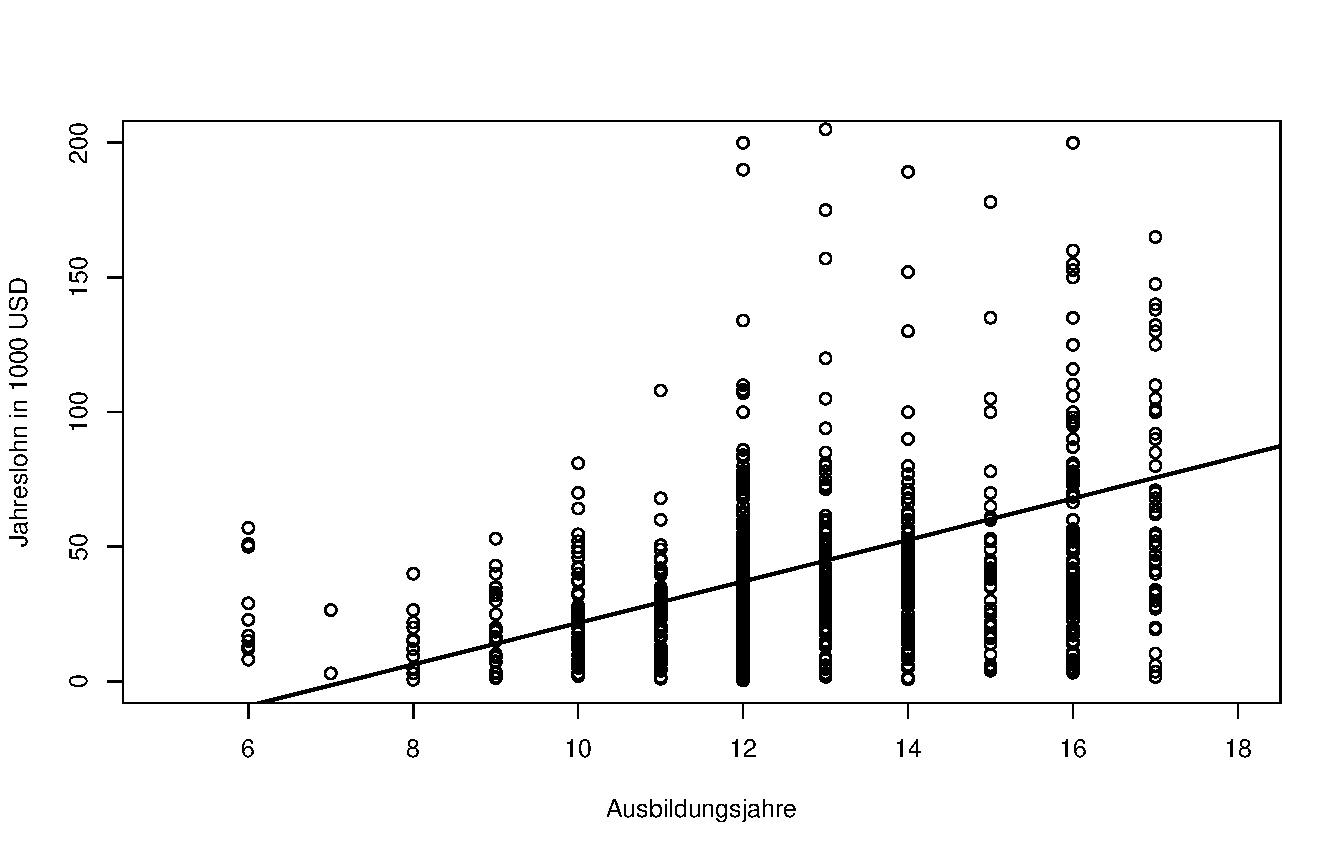
\includegraphics[height=0.4\textheight]{pics/psidwage}
	\end{center}
	\item Korrelation zwischen $Y$ und $X$ ist 0.2866
	\item Diese Information kann z.B. genutzt werden um 
	\begin{itemize}
		\item anhand von Ausbildungsjahren zu schichten
		\item Einschlusswahrscheinlichkeiten in Abhängigkeit von Ausbildungsjahren zu definieren
		\item die Schätzung effizienter zu machen
	\end{itemize}
\end{itemize}
\end{itemize}
\end{frame}

\begin{frame}{Motivation (4)}
\begin{itemize}
	\item Sekundärinformation kann sinnvoll eingesetzt werden, wenn sie folgende Eigenschaften aufweist:
	\begin{itemize}
		\item Sekundärinformation $X$ steht in einem engen Zusammenhang zur Primärinformation und interessierenden Größe $Y$
		\item Von der Sekundärinformation $X$ ist die Merkmalssumme oder der Mittelwert in der Population bekannt
	\end{itemize}
	\item Basierend auf einer Stichprobe, bekommen wir Schätzwerte für z.B. die Merkmalssummen von $X$, $\hat{t}_x$, und von $Y$, $\hat{t}_y$
	\item Intuition: Wenn wir in der Stichprobe Schätzfehler (Über- oder Unterschätzung) bei $\hat{t}_x$ machen, so werden diese auch bei $\hat{t}_y$ auftreten
	\item Der Vergleich mit dem bekannten wahren Wert $t_x$ gibt uns prinzipiell drei Möglichkeiten den Schätzer für $Y$ zu verbessern:
	\begin{itemize}
		\item Quotientenschätzer vermutet einen proportionalen Relation zwischen $X$ und $Y$
		\item Differenzenschätzer vermutet einen konstanten Shift, unabhängig vom Level von $X$
		\item Regressionsschätzer vermutet einen (nicht)linearen Zusammenhang zwischen $X$ und $Y$
	\end{itemize}
	\item Allgemein benutzen wir ein statistisches Modell für den Zusammenhang zwischen $X$ und $Y$
\end{itemize}
\end{frame}

\begin{frame}{Quotientenschätzung (1)}
\begin{itemize}
	\item Der Quotient zweier Merkmalssummen in $U$ ist
	$$ r= \frac{t_y}{t_x}$$
	\item $t_x$ ist bekannt, aber $t_y$ und somit auch $r$ sind unbekannt
	\item Basierend auf einer Stichprobe bekommen wir $\hat{t}_y$ und $\hat{t}_x$, folglich: 	$$ \hat{r}= \frac{\hat{t}_y}{\hat{t}_x}$$
	\item Für den Quotientenschätzer von $t_y$ gilt nun:
	$$\hat{t}_{y}^{ra} = \hat{r} t_x = \hat{t}_y \frac{t_x}{\hat{t}_x} = \sum_s \frac{y_k}{\pi_k}\frac{t_x}{\hat{t}_x}$$
	\item Korrektur des freien Schätzers $\hat{t}_y$ um Über- oder Unterschätzung von $t_x$ durch $\hat{t}_x$
	\item Idee: Wenn $X$ und $Y$ korreliert sind und $t_x$ in der Stichprobe überschätzt wird, so gilt dies auch für $t_y$
	\item $\hat{t}_{y}^{ra}$ ist allerdings nur asymptotisch erwartungstreu und die Varianz lässt sich auch nur approximativ berechnen
\end{itemize}
\end{frame}

\begin{frame}{Quotientenschätzung (2)}
\begin{itemize}
	\item Der Quotientenschätzer ist eine Funktion von zwei Variablen $\hat{t}_y$ und $\hat{t}_x$
	\item Approximiere $f(\hat{t}_y,\hat{t}_x)=\hat{t}_y/\hat{t}_x$ mithilfe einer Taylor Approximation:
	\begin{align*}
		\frac{\hat{t}_y}{\hat{t}_x} \approx \frac{t_y}{t_x} + \frac{1}{t_x}(\hat{t}_y-r\hat{t}_x)
	\end{align*}
	\item Einsetzen in die Quotientenschätzfunktion
	$$\hat{t}_y^{ra} = t_y + \hat{t}_y - r \hat{t}_x$$
	\item $\hat{t}_y^{ra}$ ist daher approximativ erwartungstreu, da
	$$E( t_y + \hat{t}_y - r \hat{t}_x) = t_y +t_y -\frac{t_y}{t_x}t_x = t_y$$
	\item Die approximierte Varianz ist dann
	$$AV(\hat{t}_y^{ra})=V(\hat{t}_y)+r^2 V(\hat{t}_x)-2rCov(\hat{t}_y,\hat{t}_x)$$
	
\end{itemize}
\end{frame}


\begin{frame}{Quotientenschätzung (3)}
\begin{itemize}
	\item Quotientenschätzer bei einfacher Zufallsauswahl:
	$$AV(\hat{t}_y^{ra}) = N^2\frac{1}{n}\left(1-\frac{n}{N}\right)\left(S_{y_U}^2+r^2 S_{x_U}^2 - 2r S_{xy_U}\right)$$
	\item Schätzung basierend auf einer Stichprobe:
	$$\hat{AV}(\hat{t}_y^{ra}) = N^2\frac{1}{n}\left(1-\frac{n}{N}\right)\left(S_{y_s}^2+\hat{r}^2 S_{x_s}^2 - 2\hat{r} S_{xy_s}\right)$$
	
	\item Effizienter als eine einfache Zufallsauswahl, falls $r^2S_{x_U}^2 - 2r S_{xy_U}<0$ oder
	$$ \rho_{xy} > \frac{1}{2} \frac{CV_{x_U}}{CV_{y_U}}$$
\end{itemize}
\end{frame}

\begin{frame}{Differenzenschätzung (1)}
\begin{itemize}
	\item Bei der Differenzenschätzung nehmen wir an, dass folgender Zusammenhang gilt $$y_k - x_k = \beta + \varepsilon_k$$
	\item Der Differenzenschätzer ist
	$$ \hat{t}_y^{diff} = \hat{t}_y + (t_x -\hat{t}_x)$$
	bei einfacher Zufallsauswahl
	$$ \hat{t}_y^{diff} = N \bar{y}_s + N(\bar{x}_U - \bar{x}_s)$$
	\item Der freie Schätzer $\hat{t}_y$ wird korrigiert, wenn die Stichprobe \enquote{zu große} ($t_x -\hat{t}_x<0$) bzw. \enquote{zu kleine} ($t_x -\hat{t}_x>0$) Merkmalsträger hat
\end{itemize}
\end{frame}

\begin{frame}{Differenzenschätzung (2)}
\begin{itemize}
	\item Der Differenzenschätzer ist erwartungstreu:
	$$ E(\hat{t}_y^{diff}) = E(\hat{t}_y) + E(t_x) -E(\hat{t}_x) = t_y + t_x -t_x = t_y$$
	\item Die Varianz (bei einfacher Zufallsauswahl) ist
	$$V(\hat{t}_y^{diff}) = N^2\frac{1}{n}\left(1-\frac{1}{N}\right)(S_{y_U}^2+S_{x_U}^2-2S_{xy_U})$$
	und kann geschätzt werden mit
	$$\hat{V}(\hat{t}_y^{diff}) = N^2\left(\frac{1}{n}-\frac{1}{N}\right)(S_{y_s}^2+S_{x_s}^2-2S_{xy_s})$$
	\item Effizienter als eine einfache Zufallsauswahl, falls $S_{x_U}^2 - 2 S_{xy_U}<0$ oder
	$$ \rho_{xy} > \frac{1}{2} \frac{S_{x_U}}{S_{y_U}}$$
\end{itemize}
\end{frame}

\begin{frame}{Regressionsschätzung  (1)}\small
\begin{itemize}
	\item Regressionszusammenhang als Approximation für Y: $y_k = B_1 + B_2 x_k + E_k$ 
	\item $y_k$ und $x_k$ sind für alle $N$ Elemente in $U$ fix
	\item Notation: $$X = \begin{bmatrix}1 & x_1\\1 & x_2\\\vdots & \vdots \\ 1 & x_N\end{bmatrix}, y = \begin{bmatrix} y_1\\ y_2\\ \vdots \\ y_N \end{bmatrix}, B=\begin{bmatrix}B_1\\B_2\end{bmatrix}$$
	\item Das Kleinste-Quadrate-Kriterium ist $\sum_U(y_k-x_k'B)^2$, die zugehörigen Parameter
	\begin{align*}
	B_2 &= \frac{N\left(\sum_U x_k y_k\right)-\left(\sum_U x_k\right)\left(\sum_U y_k\right)}{N\left(\sum_U x_k^2\right)-\left(\sum_U x_k\right)^2}=\frac{\sum_U\left(x_k - \bar{x}_U\right)\left(y_k - \bar{y}_U\right)}{\sum_U \left(x_k - \bar{x}_U\right)^2}\\
	B_1 &= \bar{y}_U - B_2 \bar{x}_U
	\end{align*}
	\item Der $\pi$-Schätzer basierend auf einer Stichprobe $s$ ist definiert als
	\begin{align*}
	\hat{B}_2 &=\frac{\left(\sum_s \frac{1}{\pi_k}\right)\left(\sum_s \frac{x_k y_k}{\pi_k}\right)-\left(\sum_s \frac{x_k}{\pi_k}\right)\left(\sum_s \frac{y_k}{\pi_k}\right)}{\left(\sum_s \frac{1}{\pi_k}\right)\left(\sum_s \frac{x_k^2}{\pi_k}\right)-\left(\sum_s \frac{x_k}{\pi_k}\right)^2} = \frac{\sum_s\frac{\left(x_k - \tilde{x}_s\right)\left(y_k - \tilde{y}_s\right)}{\pi_k}}{\sum_s \frac{\left(x_k-\tilde{x}_s\right)^2}{\pi_k}}\\
	\hat{B}_1 &= \tilde{y}_s - \hat{B}_2 \tilde{x}_s
	\end{align*}
	mit $\tilde{y}_s = \frac{\hat{t}_{y,\pi}}{\hat{N}}$ und $\tilde{x}_s = \frac{\hat{t}_{x,\pi}}{\hat{N}}$
	\item Bei bekannter Populationsgröße $N$ verwendet man $\tilde{y}_s=\hat{\bar{y}}$ und $\tilde{x}_s=\hat{\bar{x}}$
\end{itemize}
\end{frame}

\begin{frame}{Regressionsschätzung (2)}
\begin{itemize}
	\item Die Schätzfunktion von $\hat{B}$ basiert auf Quotienten von Zufallsgrößen, daher kein analytischer Ausdruck für Varianzen möglich
	\item Lösung: Taylor-Approximation 1. Ordnung:
	$$AV(\hat{B}_2) = \frac{\sum\sum_U \Delta_{kl}\frac{(x_k - \bar{x}_U)E_k}{\pi_k}\frac{(x_l - \bar{x}_U)E_l}{\pi_l}}{\left[\sum_U (x_k - \bar{x}_U)^2\right]^{2}}$$ mit $E_k = y_k - B_1 - B_2 x_k$
	\item Dies kann geschätzt werden basierend auf einer Stichprobe:
		$$\hat{AV}(\hat{B}_2) = \frac{\sum\sum_s \check{\Delta}_{kl}\frac{(x_k - \tilde{x}_s)e_k}{\pi_k}\frac{(x_l - \tilde{x}_s)e_l}{\pi_l}}{\left[\sum_s \frac{(x_k - \tilde{x}_s)^2}{\pi_k}\right]^{2}}$$ mit $e_k = y_k - \hat{B}_1 - \hat{B}_2 x_k$
\end{itemize}
\end{frame}

\begin{frame}{Regressionsschätzung (3)}
\begin{itemize}
	\item Im Fall der einfachen Zufallsauswahl vereinfacht sich hier einiges:
	$$\hat{B}_2 = \frac{\sum_s (x_k -\bar{x}_s)(y_k - \bar{y}_s)}{\sum_s (x_k - \bar{x}_s)^2}$$ und $\hat{B}_1 = \bar{y}_s - \hat{B}_2 \bar{x}_s$
	\item Die approximierte Varianz ist
	$$AV(\hat{B}_2) = \frac{N^2\frac{1-f}{n}\frac{1}{N-1}\sum_U (x_k - \bar{x}_U)^2 E_k^2}{[\sum_U (x_k - \bar{x}_U)^2]^2}$$
	und schätzbar basierend auf einer Stichprobe mit
	$$\hat{AV}(\hat{B}_2) = \frac{(1-f)\frac{n}{n-1}\sum_s (x_k - \bar{x}_s)^2 e_k^2}{[\sum_s (x_k - \bar{x}_s)^2]^2}$$
	\item Achtung: im stochastischen Regressionsmodel ist die Varianz des Steigungsparameter $\frac{\frac{1}{n-2}\sum_s e_k^2}{\sum_s (x_k - \bar{x}_s)^2}$ unterschiedlich groß
\end{itemize}
\end{frame}

\begin{frame}{Fazit}
\begin{itemize}
	\item Modellbasierte Stichprobenverfahren bauen auf Modellen auf, die den Einfluss der Sekundärinformation $X$ auf $Y$ beschreiben. 
	\item Das globale Modell ist dabei ein Regressionsmodell, d.h. $Y$ ergibt sich als lineare Approximation von $X$
	\item Die zu Grunde liegenden Modelle der einzelnen Schätzer lassen sich somit wie folgt schreiben:
	\begin{itemize}
\item Regressionsschätzer: $y_k = B_1 + B_2 x_k$
\item Quotientenschätzer: $y_k = B_1 + B_2 x_k$ mit $B_1 = 0$
\item Differenzenschätzer : $y_k = B_1 + B_2 x_k$ mit $B_2 = 1$
\end{itemize}
\item Es ist zu beachten, dass die Herleitung der Schätzverfahren nicht auf der Gültigkeit eines linearen Regressionsmodells als datengenerierendem Prozess basiert, sondern nur die Regressionsgerade der Grundgesamtheit als Hilfsmittel benutzt.
\item Lineare Regressionsmodell wird hier nicht mit den üblichen Modellannahmen verwendet wird, sonder für die \enquote{modellunterstützte (model assisted)} Schätzung.
\end{itemize}
\end{frame}
\end{document}